\chapter{Graphene}
\label{ch:graphene}
Graphene is one of the most studied materials ever. It consists of a two-dimensional array of $C$ atoms arranged in a honeycomb lattice like that of the Fig.~\ref{graphene_structure}~($a-d$). The honeycomb lattice is not a Bravais lattice so in order to describe such a system (in terms of Bloch functions) we can choose a wide variety of unit cells and lattice vectors. The simplest choice is the two atoms unit cell with a triangular Bravais lattice as shown in Fig~\ref{graphene_structure}~(a). Nevertheless any other choice of unit cell and lattice vectors is valid as long as it tessellates the space. %XXX
%~~~~~~~~~~~~~~~~~~~~~~~~~~ FIGURE ~~~~~~~~~~~~~~~~~~~~~~~~~%
\begin{figure}[h!]
\centering
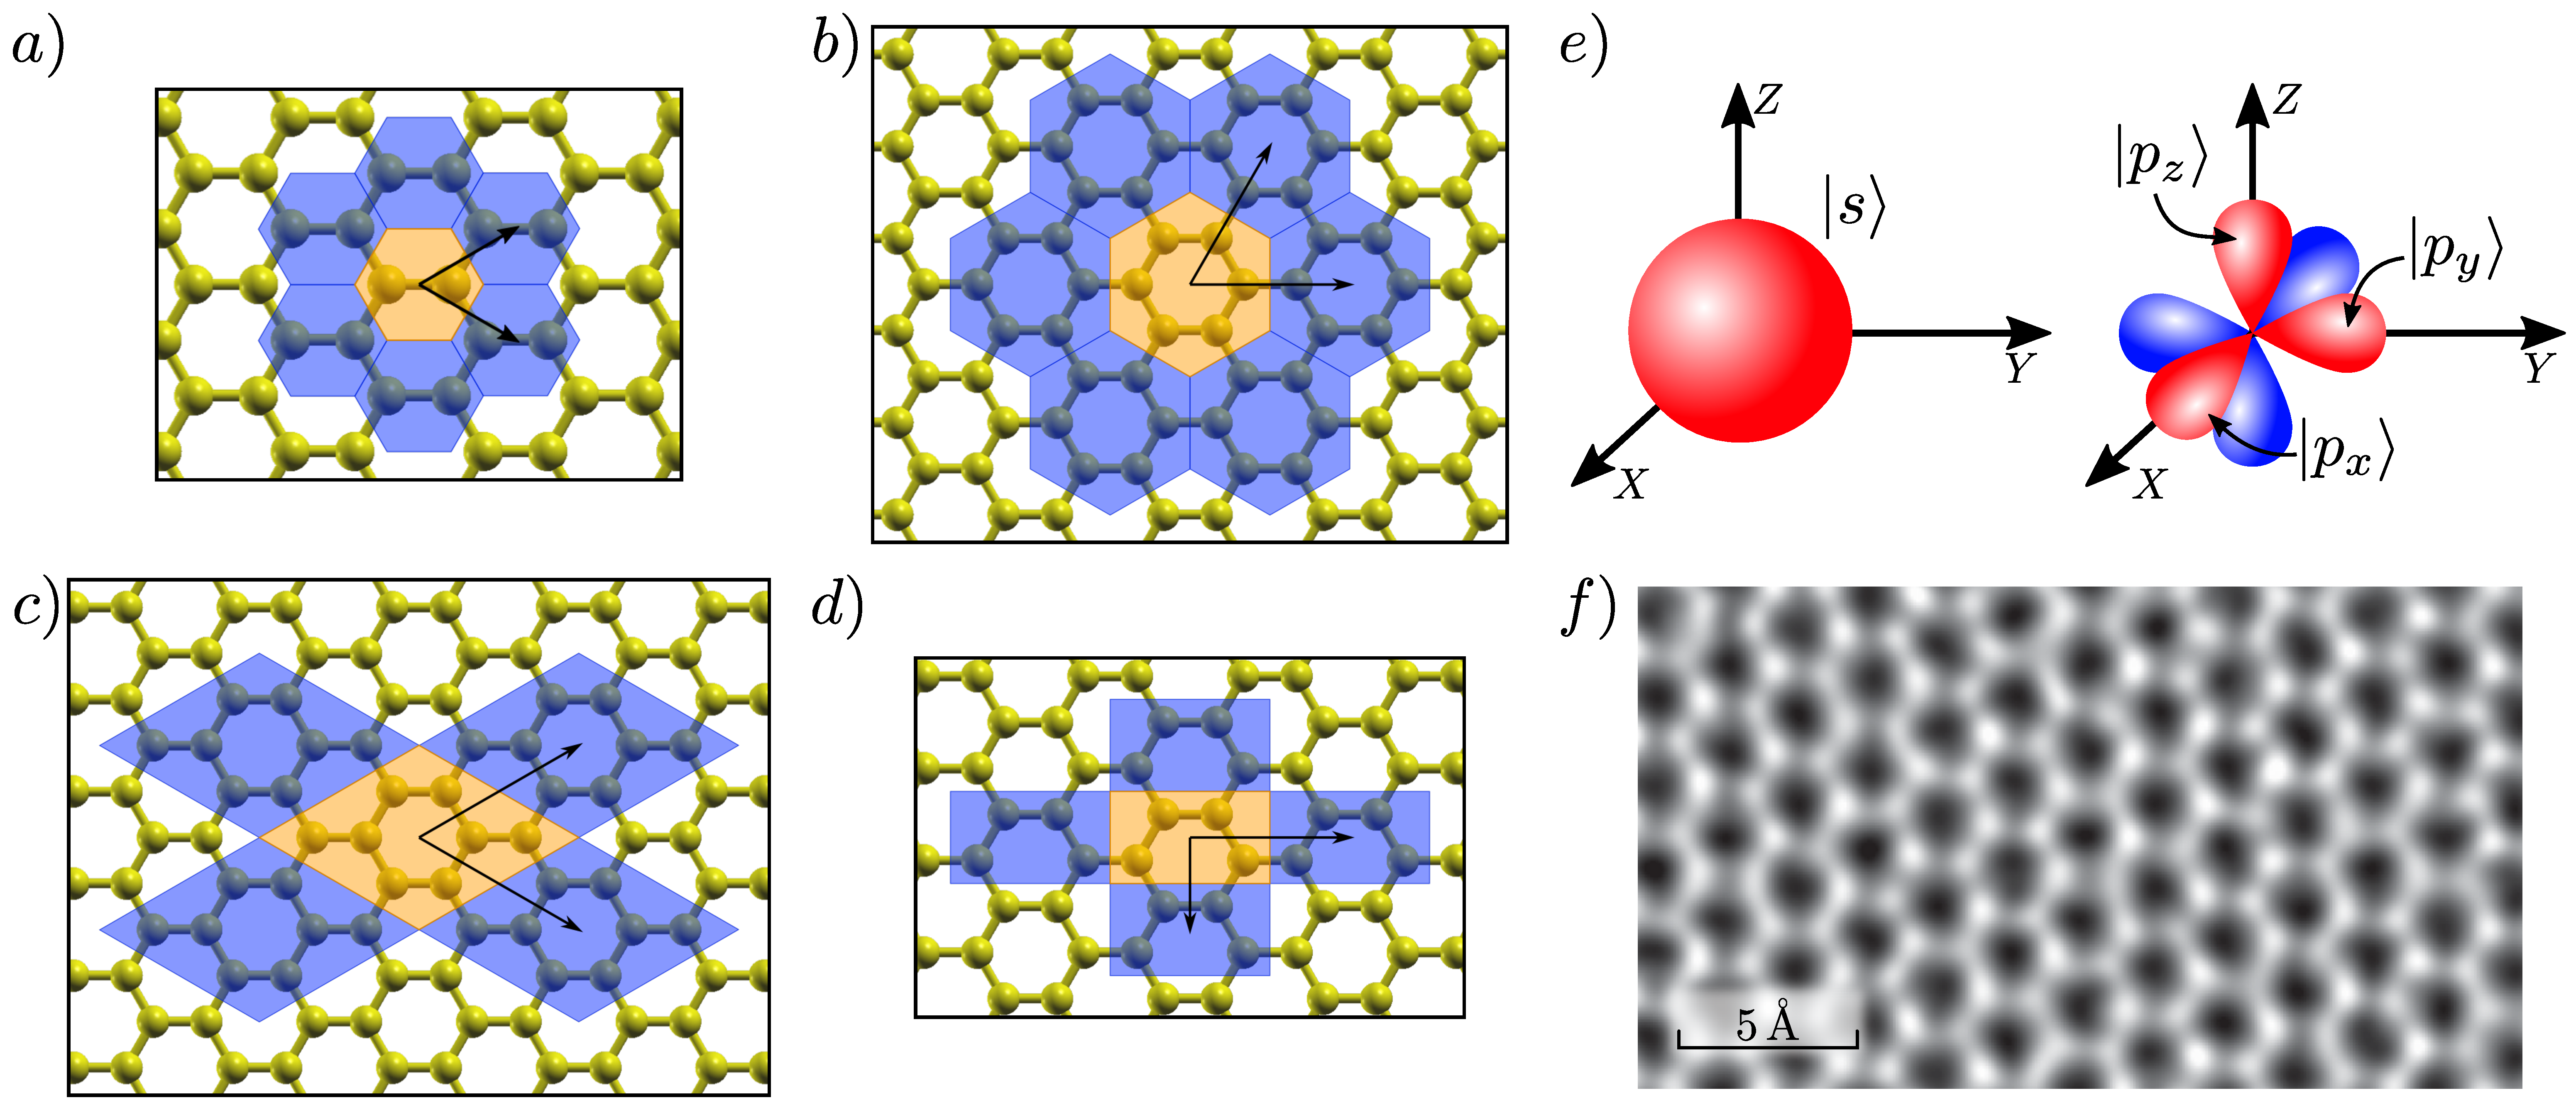
\includegraphics[width=\textwidth]{chapter04/figures/graphene.pdf}
\vspace{-5pt}
\caption{$(a-d)$ Graphene atomic structure considering differnt unit cells and lattice vectors. $(e)$ relevant hydrogenic orbitals for the $C$ atom.}
\label{graphene_structure}
\end{figure}
\FloatBarrier
%~~~~~~~~~~~~~~~~~~~~~~~~~~~~~~~~~~~~~~~~~~~~~~~~~~~~~~~~~~~%
Carbon atoms have 6 \ac{el}, 2 in the 1s level, 2 more in the 2s level and finally another 2 \ac{el} in the 2p level. Since the orbitals $n=1$ are full and very far in energy there is no need to consider them.
The 2s level is also full, but not so far from the Fermi energy, so we will take a look at its importance.
We will study the 2p orbitals in two groups since the $p_z$ orbital has no hopping to the other $p$ orbitals due to mirror symmetry (Fig.~\ref{graphene_structure}~(e)).
%TODO



\section{Slater-Koster tight-binding model}
\label{sec:SK}
Generally the hopping parameters are an input in any \ac{tb} model, and usually they are calculated by fitting eigenvalues and eigenfunctions obtained from \ac{dft} calculations (the eigenfunctions are usually projected to a basis of localized atomic orbitals) or by fitting experimental data.

As a system grows complex, more and more parameters are needed to describe it, nevertheless since the number of different orbitals is finite, one could expect that not all the parameters are completely independent from the others.


The \ac{sk} approximation takes into account the symmetry of the orbitals to reduce the number of parameters needed. Due to the symmetry of the atomic orbitals it is to be expected that different hoppings could be related. It is easier to see this point with an example.
%~~~~~~~~~~~~~~~~~~~~~~~~~~ FIGURE ~~~~~~~~~~~~~~~~~~~~~~~~~%
\begin{figure}[h!]
\centering
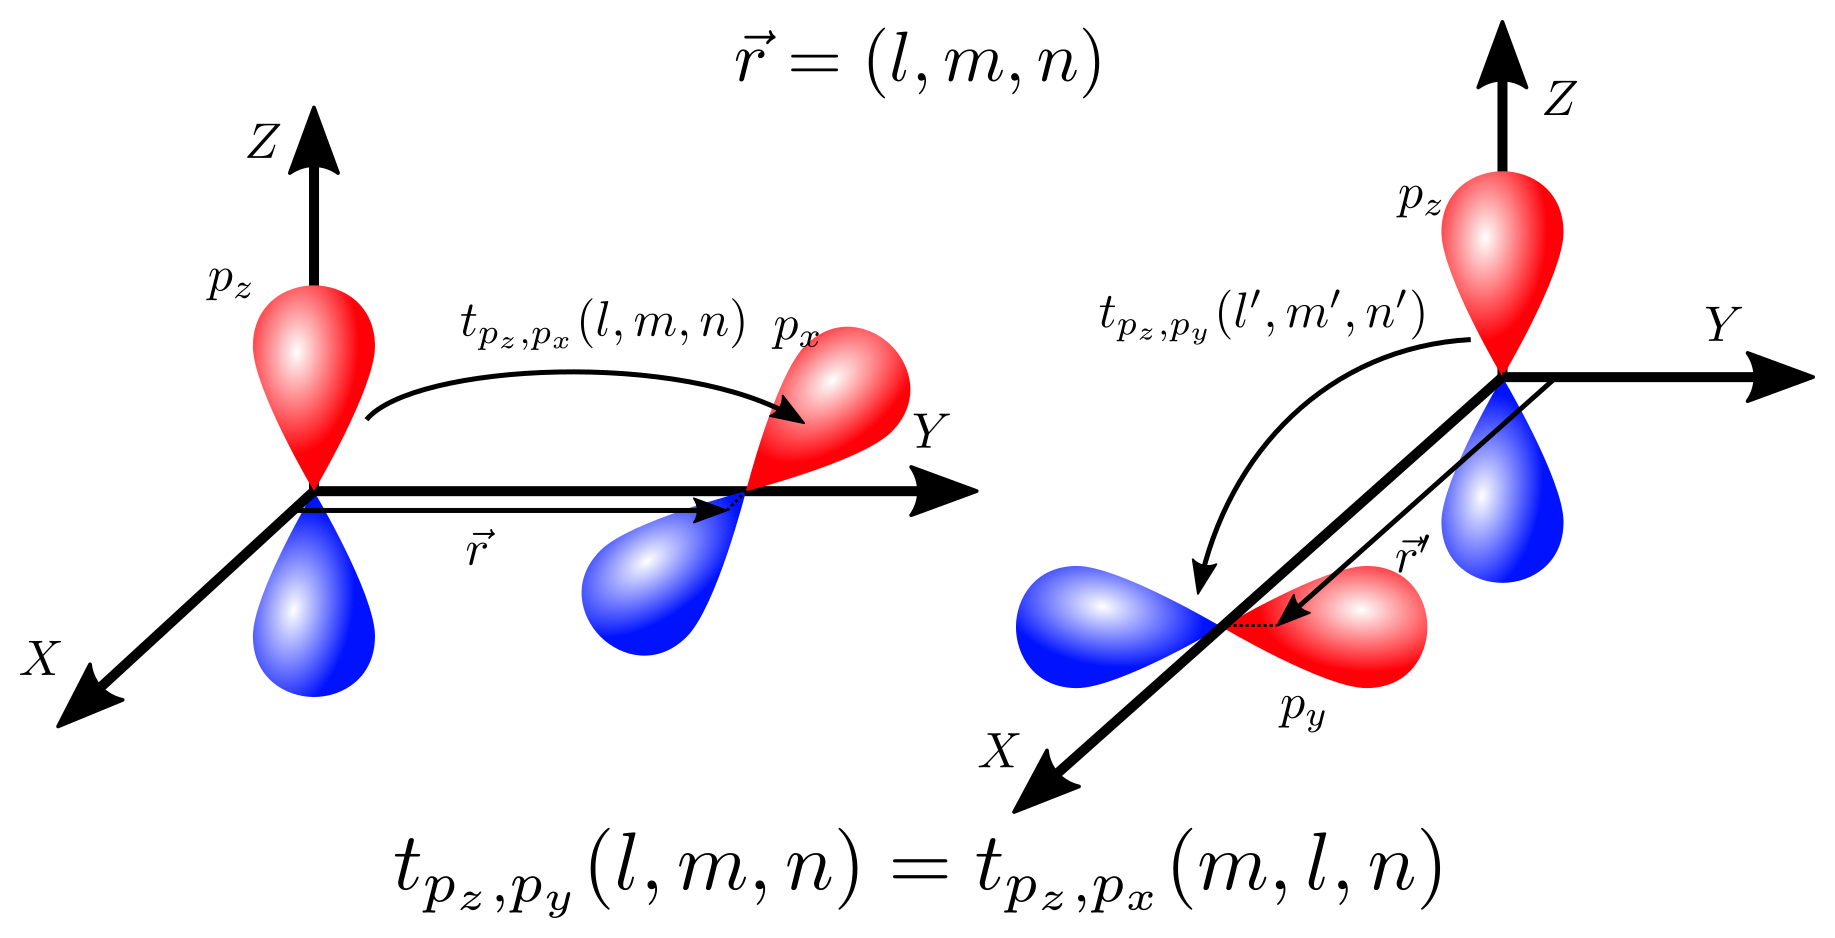
\includegraphics{chapter04/figures/complex.png}
\vspace{-5pt}
\caption{Relation between $t_{p_{z},p_{x}}$ and $t_{p_{z},p_{y}}$ hopping. In this case we need not only to rotate each orbital but also the position of the atoms, but it is clear that one hopping can be calculated from the other.}
\label{complex}
\end{figure}
\FloatBarrier
%~~~~~~~~~~~~~~~~~~~~~~~~~~~~~~~~~~~~~~~~~~~~~~~~~~~~~~~~~~~%
In figure~\ref{complex} we can see that the hoppings $t_{p_{z},p_{x}}$ and $t_{p_{z},p_{y}}$ are in fact related by a rotation of the system, and we could expect that they would be functionally equal.
If we define the unitary vector $\hat{r} = \vec{r}/|\vec{r}|$ and call its components $l$, $m$, $n$, ($\hat{r}=(l,m,n)$) we can see that
\begin{equation}
  t_{p_{z},p_{x}} (l,m,n) = t_{p_{z},p_{y}}(m,l,n)
\end{equation}
notice that the change in the arguments is equivalent to perform a rotation of the vector $\vec{r}$ of $-\pi/2$ around the $Z$ axis, as shown in Fig.~\ref{complex}.

By doing this kind of transformations we can see that all the ($p-p$) hoppings can be decomposed in just two kinds of bonds depending on the relative orientation of the orbitals. This is illustrated in figure~\ref{bonds}.
%~~~~~~~~~~~~~~~~~~~~~~~~~~ FIGURE ~~~~~~~~~~~~~~~~~~~~~~~~~%
\begin{figure}[h!]
\centering
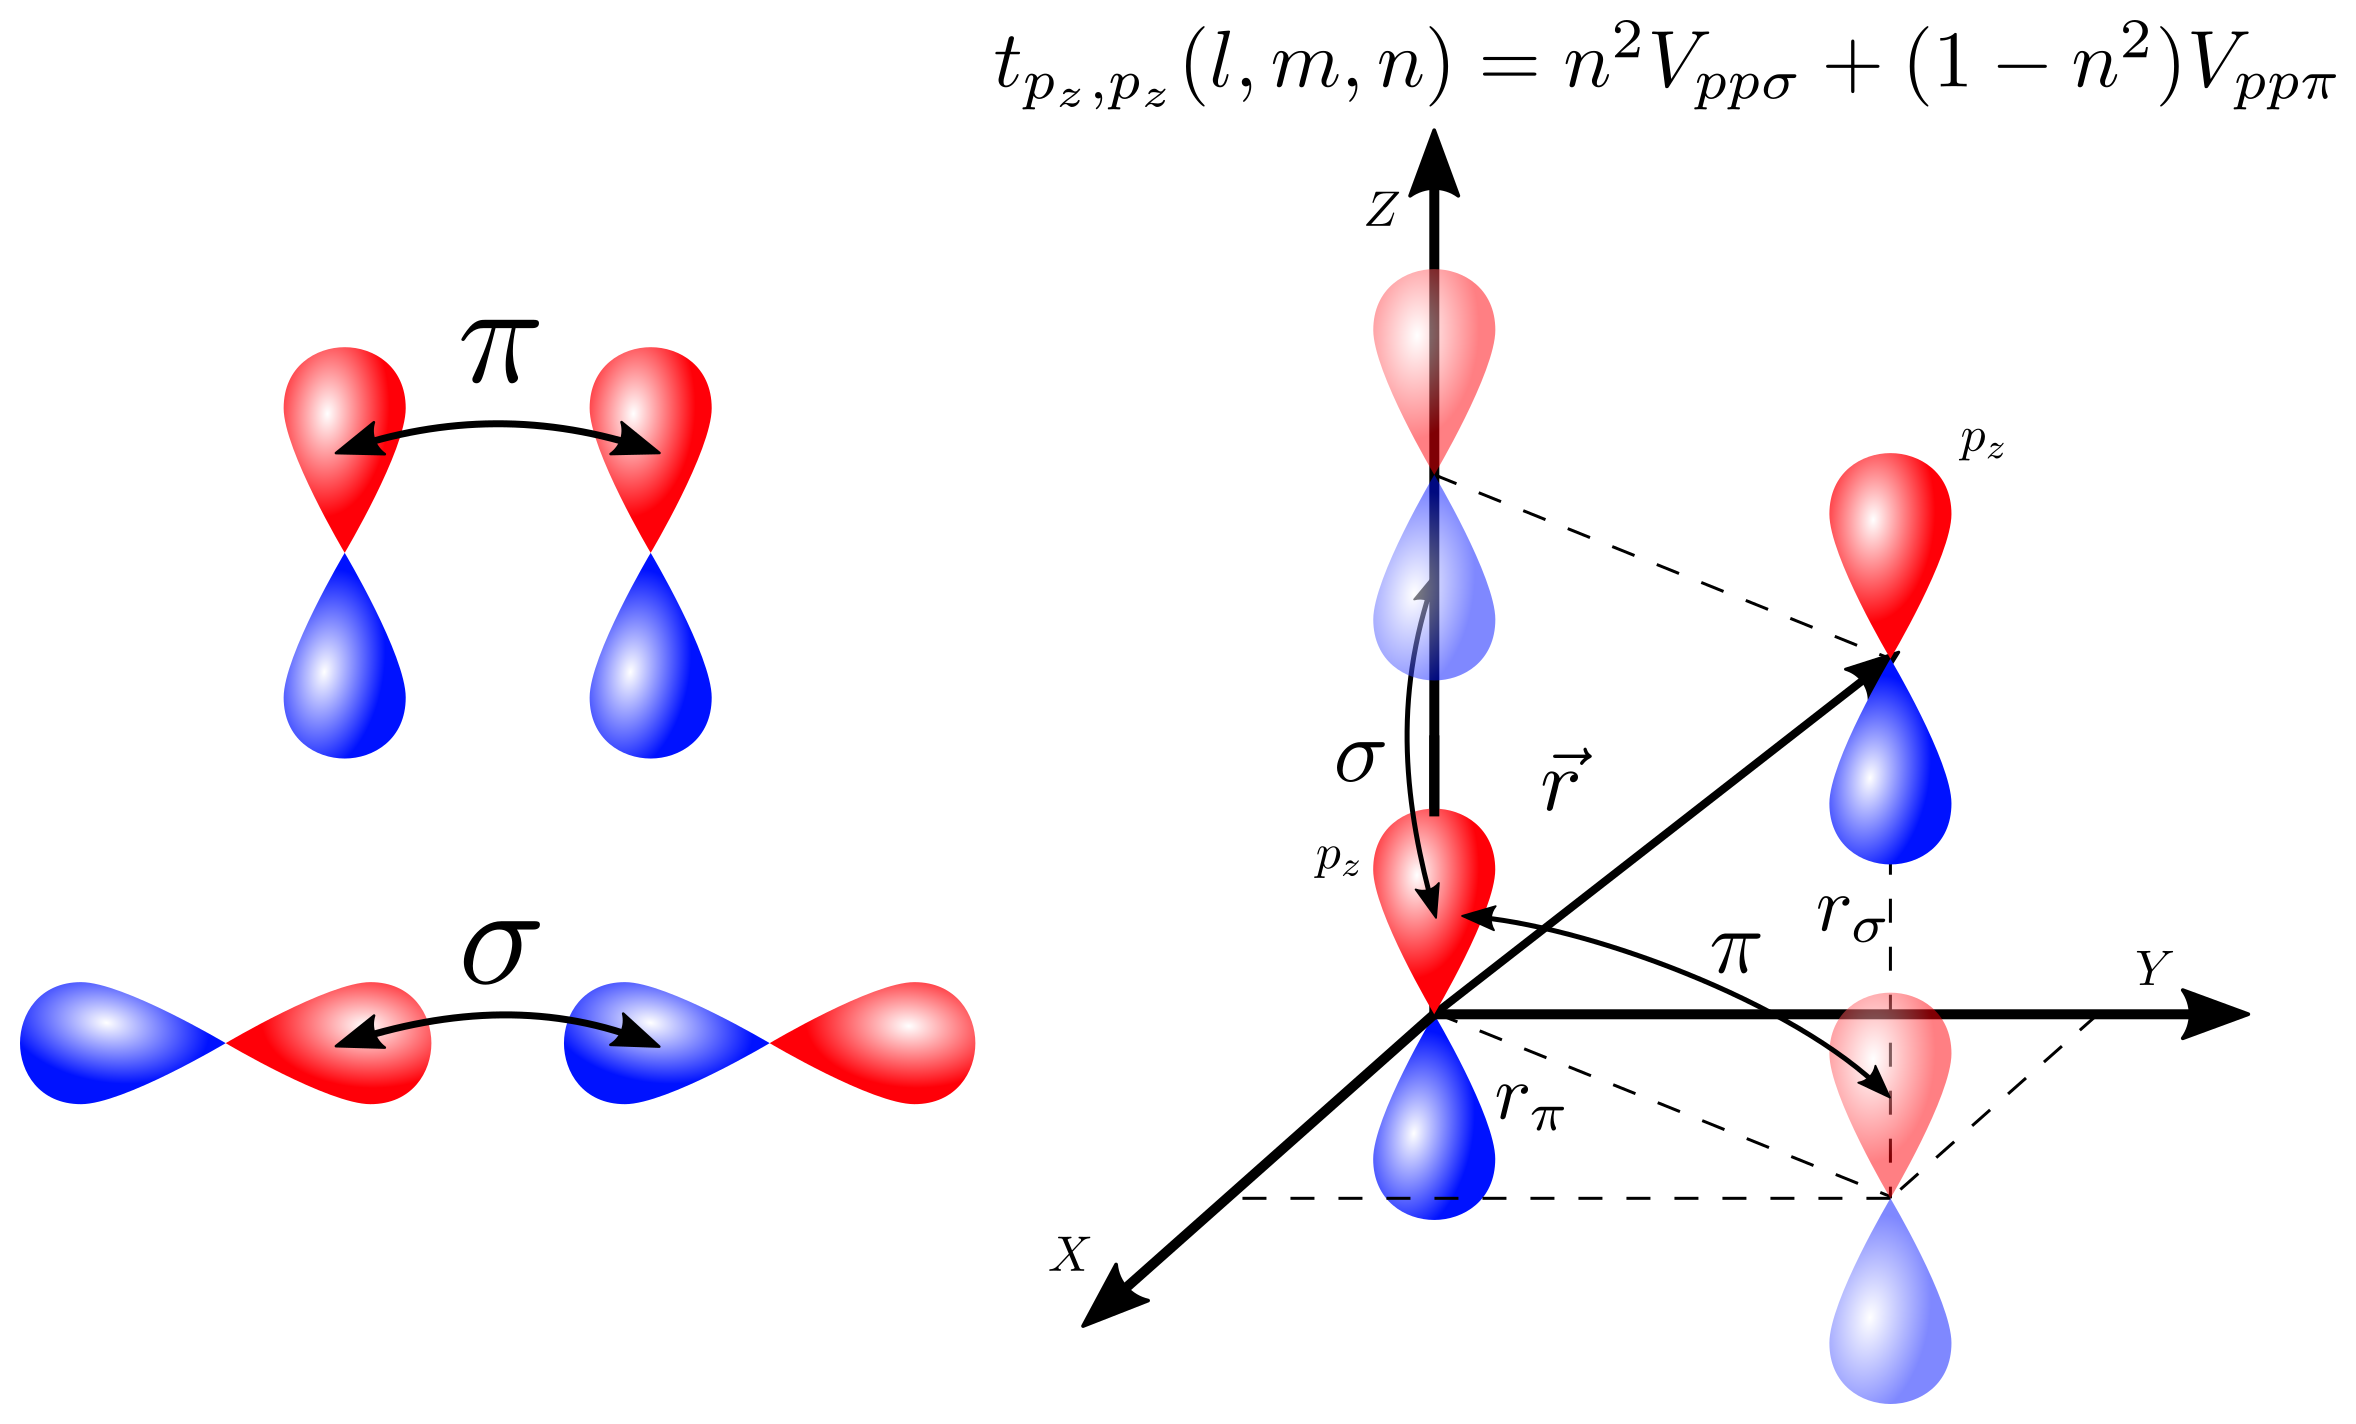
\includegraphics{chapter04/figures/bonds.png}
\vspace{-5pt}
\caption{$a)$ Only two different types of bonds between $p$ orbitals. $b)$ Simplification of the \ac{sk} hopping parameter by decomposing the hopping into its $\sigma$ and $\pi$ component, in this case it is easy to see that the hopping from any $p_{z}$ orbital to another one that in the $XY$ plane will be purely a $\pi$ bond.}
\label{bonds}
\end{figure}
\FloatBarrier
%~~~~~~~~~~~~~~~~~~~~~~~~~~~~~~~~~~~~~~~~~~~~~~~~~~~~~~~~~~~%
We can notice that in the case of graphene, where close to the Fermi energy the only involved orbitals are $p_{z}$ and, since all the hoppings are in-plane ($n=0$), all the bonds will be purely $\pi$ bonds, just because of the symmetry of the orbitals.\\


In the \ac{sk} approximation the atomic distances are encoded in the magnitude of the bonds, $V_{ss\sigma}$, $V_{sp\sigma}$, $V_{pp\sigma}$, $V_{pp\pi}$ (we will call them simply \ac{sk} parameters for short). The coefficients ($l$, $m$, $n$) in the analytic formulas are the responsible for capturing the symmetries arising both form the orbital (sign) and from the atomic structure (direction).\\

This decoupling of magnitude and direction in the hoppings provides a simple model able to capture the effects of geometric deformations, and any symmetry (breaking) in the atomic structure. For instance the effect of buckling in graphene is easily captured by this model.\blue{bands, bands with buckling,...}

\red{explain better}
The effect due to a reduction/increase of the hopping would be included by modifying the \ac{sk} parameters, yet the dependence of this parameters with the interatomic distance is not always easy to calculate.\\

At the end of the day the \ac{sk} approximation results in a reduction of the parameters needed to describe the hoppings in the system. For example, in a system with $s$, $p_x$, $p_y$, $p_z$, $d_{xy}$, $d_{yz}$, $d_{zx}$, $d_{x^{2}-y^{2}}$ and $d_{3z^{2}-r^{2}}$ we would expect 36 parameters to describe all the different hoppings, but within the \ac{sk} approximation we would only need 10 parameters.\\


The main drawback for the \ac{sk} model is to actually obtain the \ac{sk} parameters. In fact it is not guaranteed (at all) that for any given system a set of \ac{sk} parameters should exist.
Knowing that this approximation is based upon the symmetry of the atomic orbitals it is expected that for systems where the atomic orbitals are heavily hybridized this description will not suffice.

\red{Discussion limits, covalent, deformation, localized orbitals}



\section{Physical properties of Graphene}
\subsection{Bands}
Here some bands with Slater-Koster, maybe include bismuth, BN, Zeeman, SOC...
%~~~~~~~~~~~~~~~~~~~~~~~~~~ FIGURE ~~~~~~~~~~~~~~~~~~~~~~~~~%
\begin{figure}[h!]
\centering
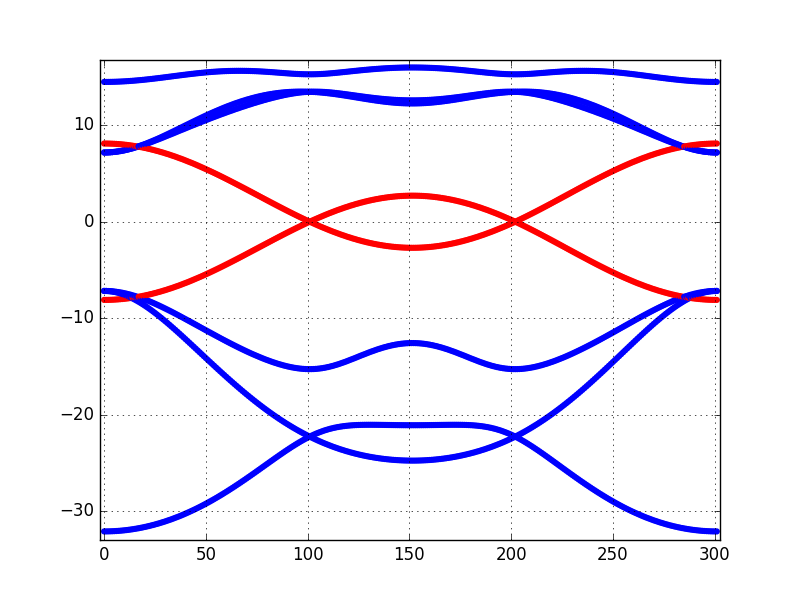
\includegraphics{chapter04/figures/graphene_bands.png}
\vspace{-5pt}
\caption{Graphene bands in the \ac{sk} approximation, with $s$, $p_x$, $p_y$, $p_z$ orbitals for the $C$ atoms. The color denote the $p_z$ component of each state. It can be seen that the $p_z$ orbital are decoupled from the rest of the orbitals and at low energy they are enough to describe the system}
\label{Gbands}
\end{figure}
\FloatBarrier
%~~~~~~~~~~~~~~~~~~~~~~~~~~~~~~~~~~~~~~~~~~~~~~~~~~~~~~~~~~~%

\subsection{Quantum Spin Hall}
\ac{qsh} in multilayers
